% -*- mode: latex; -*-
\svnid{$Id: Overview.tex 25 2008-05-28 11:56:36Z ahija $}
\section{General overview} \label{Overview}
\subsection{Process chain}
\label{Process_chain}
\begin{figure}[hbtp]
 \centering
 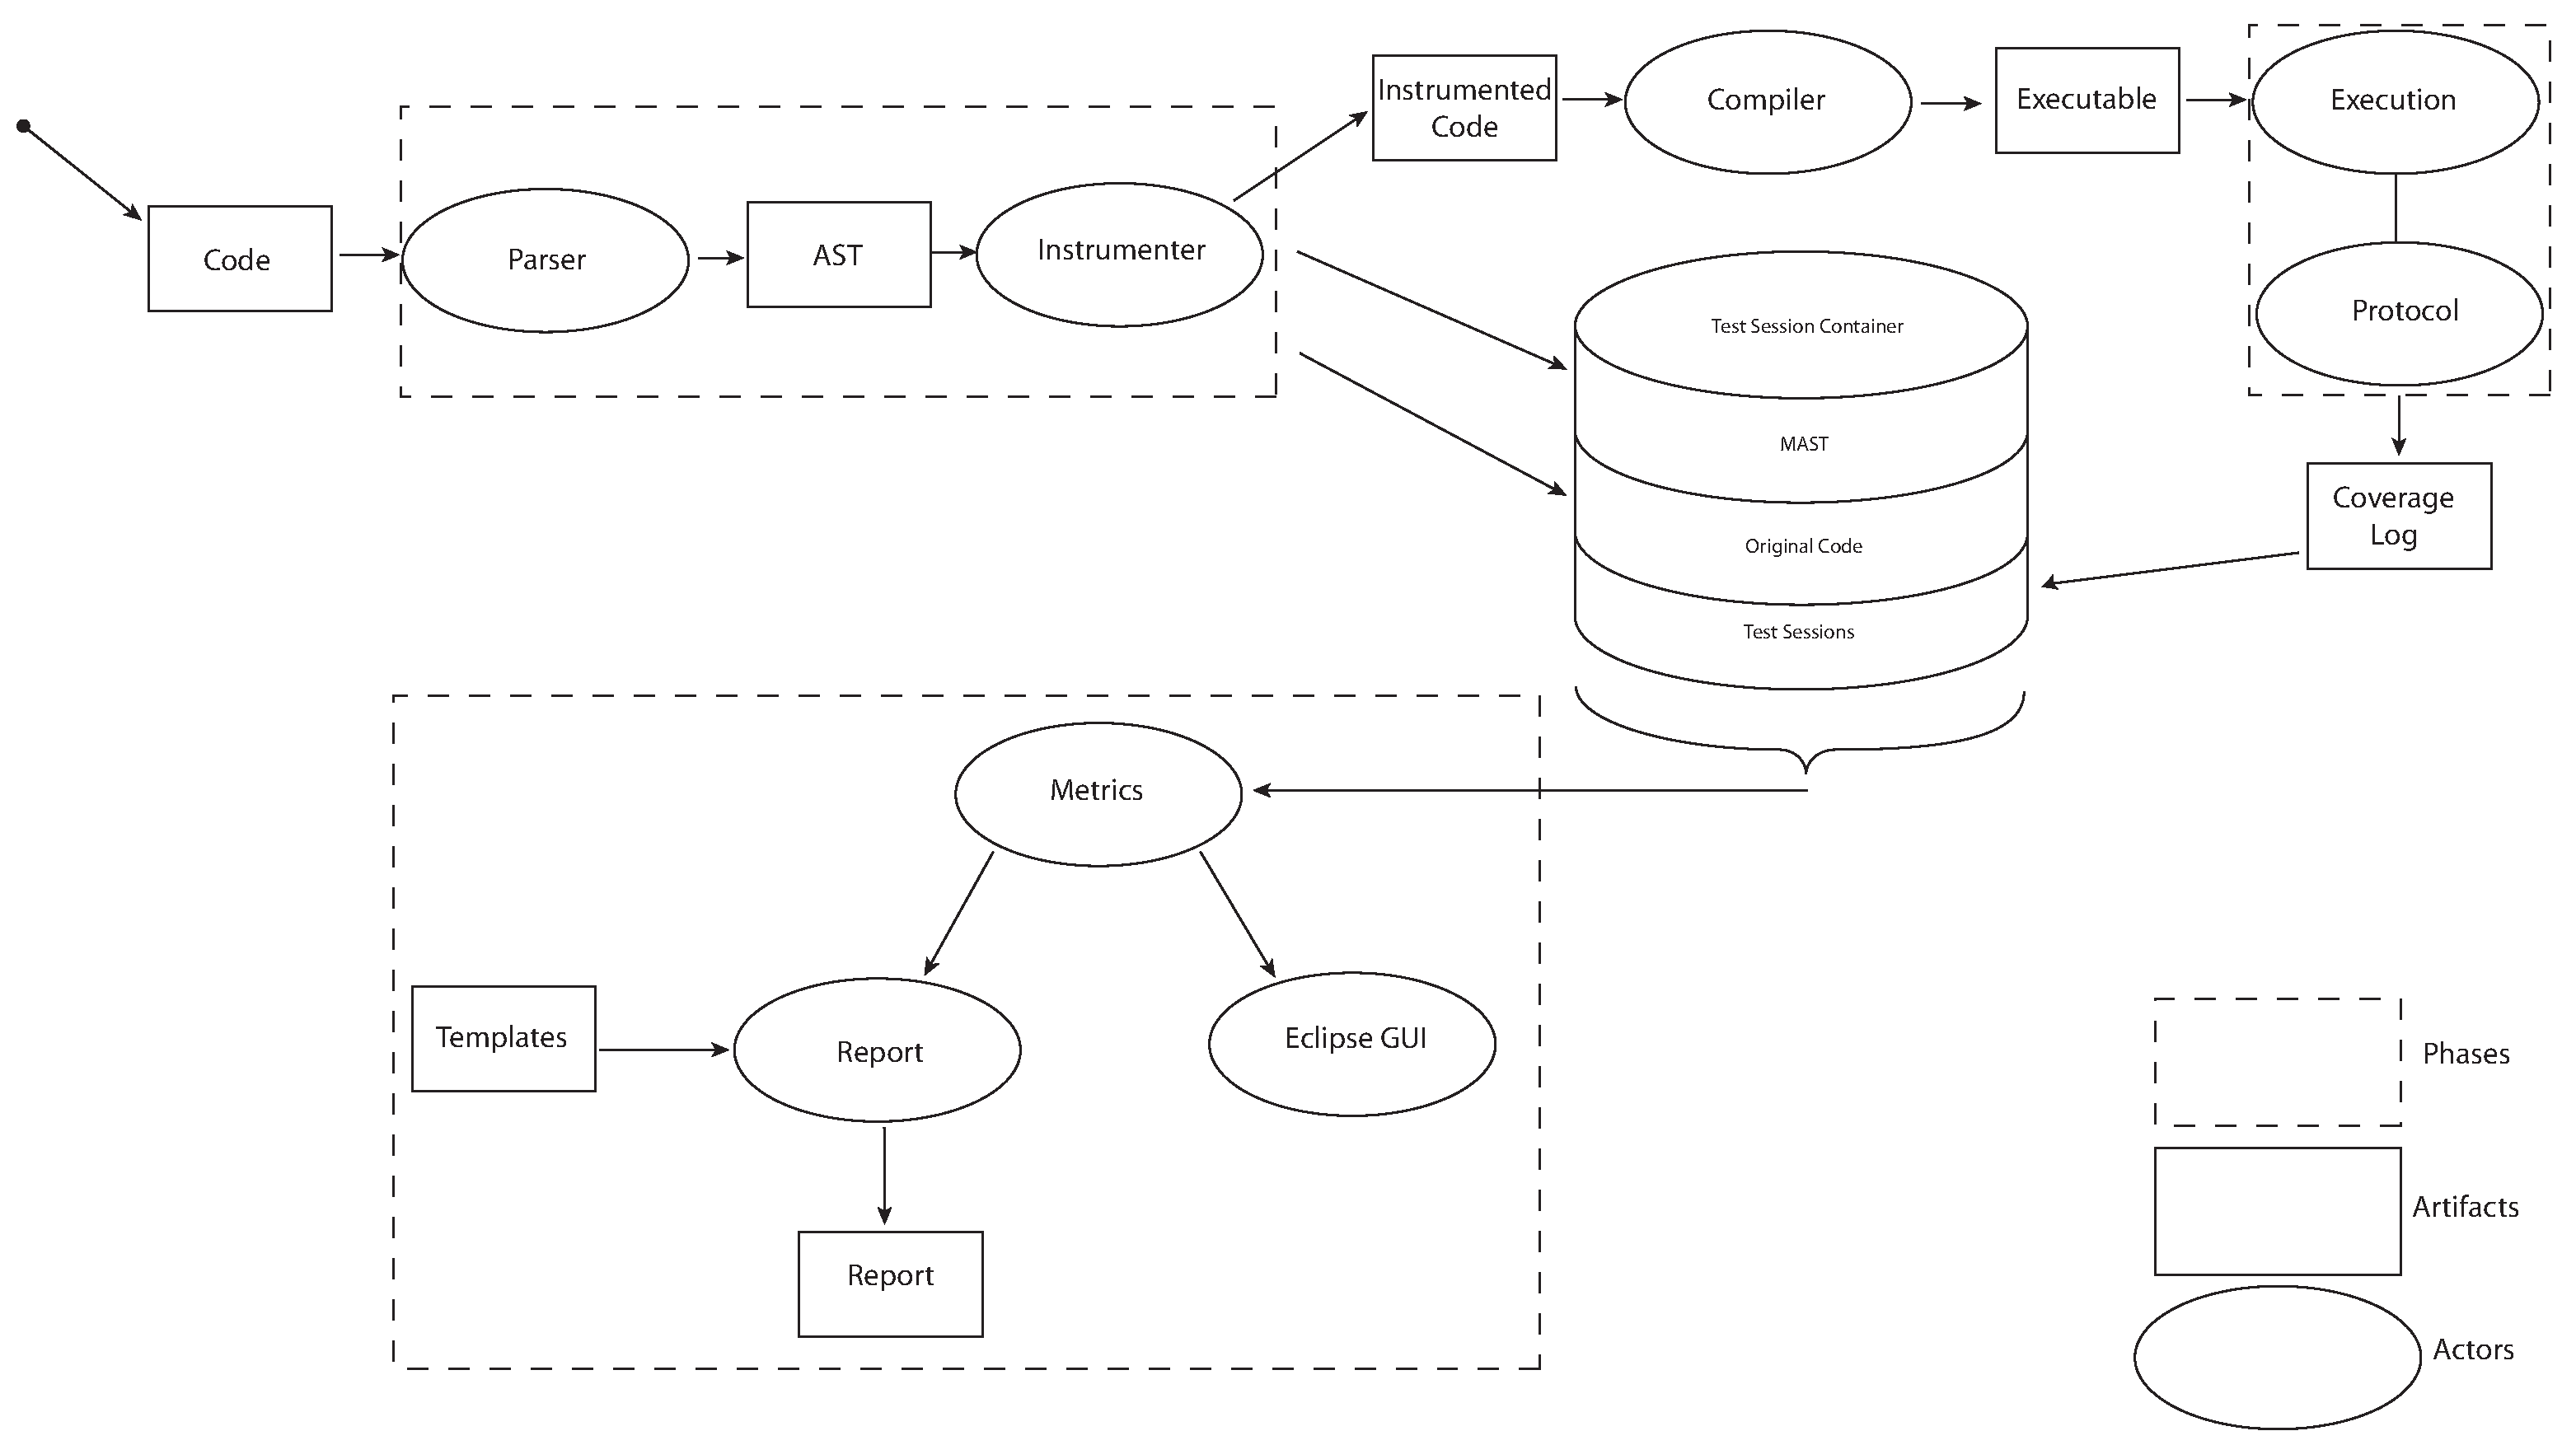
\includegraphics[width=\textwidth]{images/Overview/process_chain.pdf}
 \caption{Process chain}
 \label{figure:Overview:process_chain}
\end{figure}

This section describes the process of \gbt in detail. The whole process consists
of three phases: instrumentation, execution and reporting. Each phase includes
actions which are performed and which create certain artifacts. The arrows in
figure \ref{figure:Overview:process_chain} denote the data flow between the actors.
\par
The process starts in the instrumentation phase and the only required input is a
set of valid code files (can be compiled without getting an error message). The
instrumenter consists of a parser and a part which performs the actual
instrumentation of the source code. The parser is generated automatically from
 a javacc grammar with the help of the Java Tree Builder (JTB). This needs to be
done only once, e.g. when the instrumenter is built.
\par
This parser
 creates an abstract syntax tree (AST) representation of the source code file. The
 actual instrumentation is performed by traversing this AST and adding additional
 code to create an instrumented version of the code. During this traversal the 
static information about the code is collected and the modified abstract syntax tree
(MAST) is 
created. The MAST is a model of the source code containing only
the elements of the source code which are necessary to calculate coverage criteria
 e.g. statements, branches or boolean expressions which have an effect on control
flow. The MAST is language independent. Every element in the
MAST also contains a reference to its location in the corresponding
source code file. Both the original code and the generated MAST
are saved in the Test Session Container. 

After the code is instrumented, executable code can be generated by a compiler. This has to be done by the user if the CLI is used. The compiling is initiated and controlled by \gbt when using the Eclipse Plugin. But compilers are not part of \gbt. The required compilers must be installed separately.

Then the instrumented code can be executed and the coverage measurements will be recorded into the coverage log separated by test cases. The coverage log is saved in the Test Session Container. It holds the information on the number of executions of a coverable item in case of statement coverage, branch coverage and loop coverage or the assignments which were assigned to boolean terms in case of condition coverage.

Now the Test Session Container contains all information which is needed to calculate coverage metrics:
\begin{itemize}
 \item the MAST which is needed to connect the results of the coverage measurement in the coverage log to specific elements in the code
 \item the original code which is needed to generate reports with code highlighting
 \item the coverage log which contains the coverage measurements
\end{itemize}
Thus the coverage metrics can be calculated for report generation or to be output to the Eclipse GUI.

For report generation the structure of the code is retrieved from the MAST. Since the information in the MAST is independent from programming language, the implementation of report generation is also independent from the programming language. Report generation happens based on test cases and a template which defines the design and output format (e.g. HTML) of a report. By specifing test cases the coverage measurements, the report is based on, can be limited. Since the coverage log contains the coverage metrics separated by test cases, these metrics can be calculated and used in the report.
\subsection{Adding support for new programming languages}
\label{Adding_new_languages}
In order to add support for a new programming language a new instrumenter needs
to be written. If a javacc grammar is available for the language the parser can
be easily generated with JTB. Then a component which performs the actual
instrumentation needs to be written, which adds the necessary instrumentation code
and creates the MAST. %Depending on how the coverage log is generated
A component for logging needs to be supplied too. Everything else of \gbt is
not language dependent and requires no further action.


\section{Component overview}\label{Component_Overview}

\begin{figure}[hbtp]
 \centering
 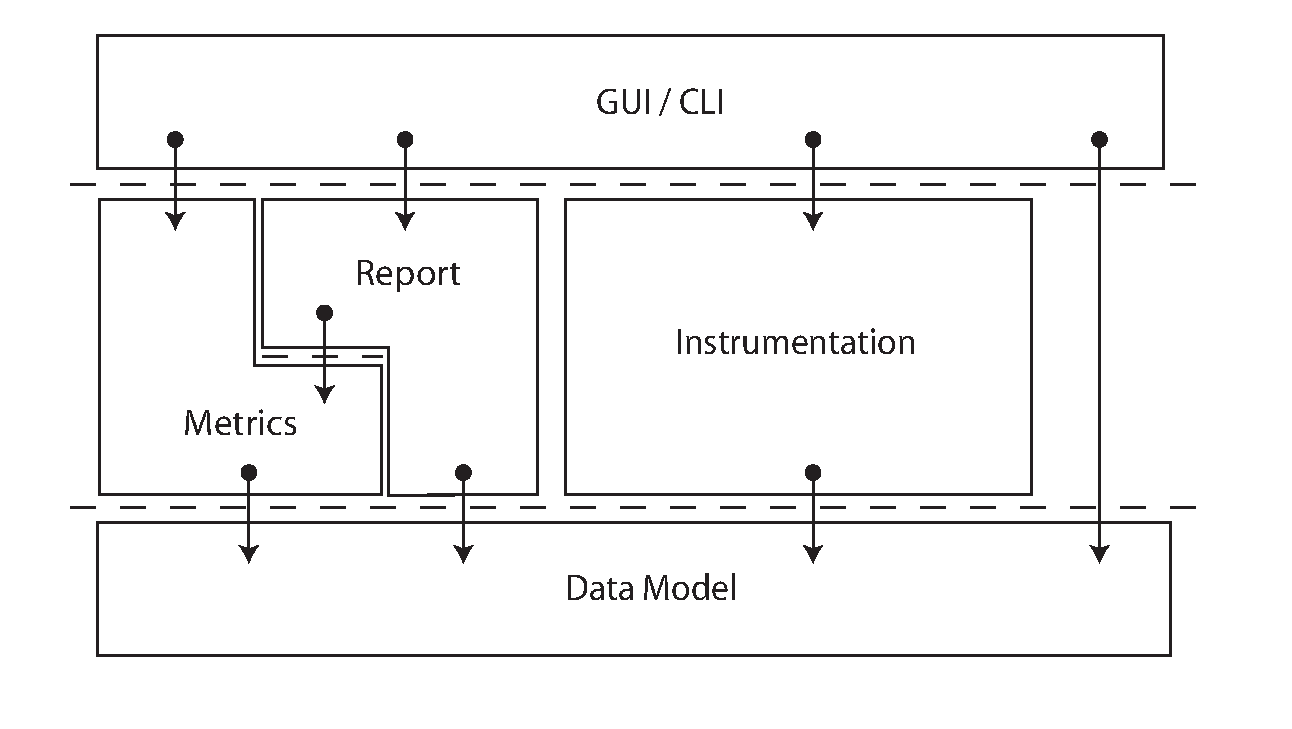
\includegraphics[width=0.8\textwidth]{images/Overview/components_layered.pdf}
 \caption{Component overview}
 \label{figure:Overview:component_diagram}
\end{figure}
As can be seen in Figure~\ref{figure:Overview:component_diagram}, the software consists of five general components, which are arrayed in a hierarchical fashion. The arrows leading from one component to another symbolize an \textit{accessing} relationship, which runs from top to bottom. The \code{Data Model} is situated at the bottom, since it acts as the foundation for all other components. On top of the data model are the components \code{Instrumentation}, \code{Report} and \code{Metrics}, with the last one also being accessible by the \code{Report} component. The topmost layer is the user interface, be it a graphical user interface (\code{GUI}), or a commandline interface (\code{CLI}).

\subsection{Data model}
This component contains all the packages and classes that are needed to hold the data generated by the instrumentation itself and the data resulting from the execution of an instrumented SUT. Every other component has access to the data model.

%\subsubsection{AST}
%\namespace{\pkg{\rootpkg.model.ast}}

The following classes are used to represent the AST. The data will be stored in
XML files. A description of the format of these XML files can be found in
 the detailed design document.
 % , however this fact is hidden by the data model and
%can be changed to a DB-based design in the future.

\begin{figure}[hbtp]
 \centering
 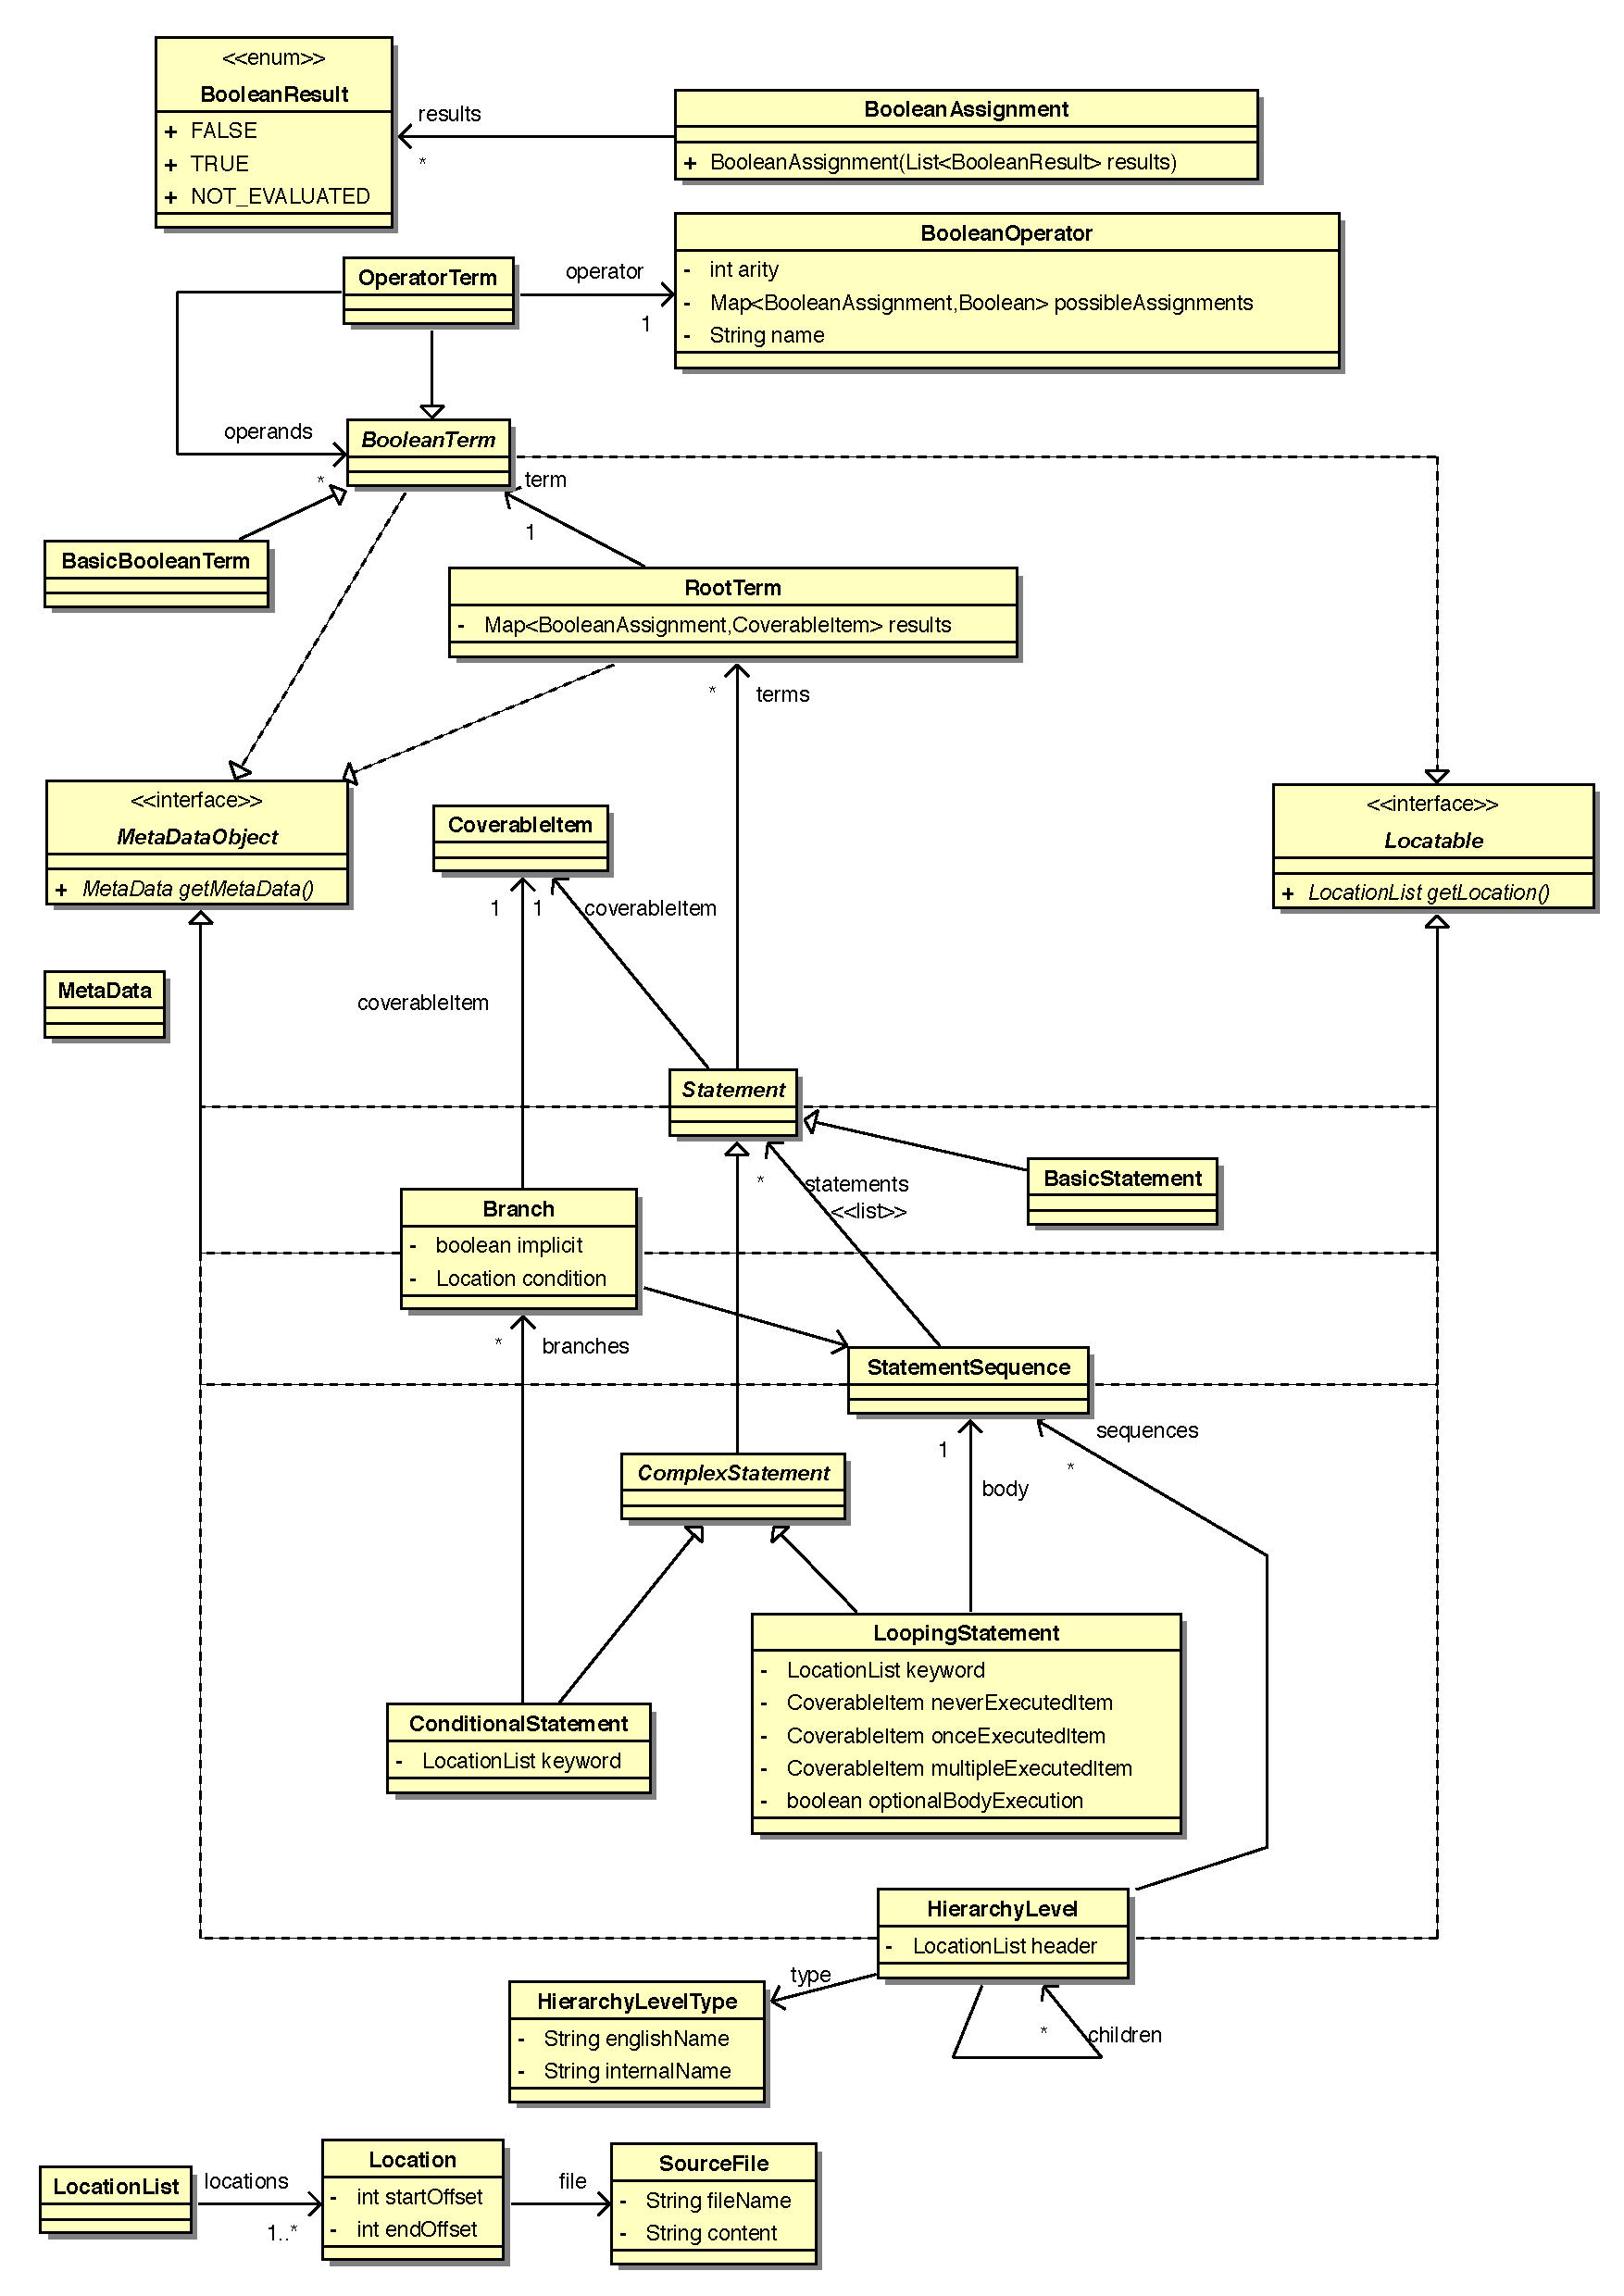
\includegraphics[height=\textheight]{images/Model/ast.pdf}
 \caption{\pkg{\rootpkg.model.ast}}
 \label{figure:Classes:Model:AST}
\end{figure}

%\pkg{\rootpkg.model.ast} has classes to represent the abstract syntax tree
%(AST) of the system under test.

\subsubsection[MetaDataObject]{\itf{MetaDataObject}}

\itf{MetaDataObject} is implemented by all classes to which meta data can be
associated.

It has only one method (\mtd{getMetaData()}) which can be used to get the
\cls{MetaData}.

Instances of this class can be passed to the methods
\mtd{setObjectMetaData(...)} and \mtd{getObjectMetaData(...)}
of the class \cls{TestCase}.

\subsubsection[MetaData]{\cls{MetaData}}

A \obj{MetaData} represents the meta data associated to a AST element,
e.g. coverage data linked to certain elements of the AST.

This class is used internally.

\subsubsection[CoverableItem]{\cls{CoverableItem}}

A \obj{CoverableItem} represents a coverable item which can be covered in
a test case.

Instances of this class can be passed to the method \mtd{getCoverageCount(...)}
of the class \cls{TestCase}.

\subsubsection[Locatable]{\itf{Locatable}}

A \imp{Locatable} is an object with one or multiple locations.

The method \mtd{getLocation()} can be used to get this locations.

\subsubsection[LocationList]{\cls{LocationList}}

A \obj{LocationList} is a list of \obj{Location}s.

This is necessary since some AST elements can have mulitple locations
(e.g. a \code{partial class} in C\#).

\subsubsection[Location]{\cls{Location}}

A \obj{Location} is a segment in a code file.

It is given by its \fld{startOffset} (which is the offset of the
first \code{char} belonging to the location), its \fld{endOffset}
(which is the offset of the first \code{char} no longer belonging to the
location), and the file which contains this location.

\subsubsection[SourceFile]{\cls{SourceFile}}

A \cls{SourceFile} represents a source file.

It contains the \fld{fileName} and the \fld{content} of the file.

\subsubsection[BooleanResult]{\cls{BooleanResult}}

A \obj{BooleanResult} is an \code{enum} which describes the result of the
evaluation of a boolean term.

The value \code{NOT\_EVALUATED} is used if a subterm was not evaluated, e.g.
because of the short circuit behaviour of an operator.

\subsubsection[BooleanAssignment]{\cls{BooleanAssignment}}

A \obj{BooleanAssignment} assigns every basic boolean term of a boolean term
an \obj{BooleanResult}.

\subsubsection[BooleanTerm]{\clsab{BooleanTerm}}

A \obj{BooleanTerm} represents a boolean term which ist constructed of basic
boolean terms and boolean operators.

A \obj{BooleanTerm} can be a \cls{BasicBooleanTerm} or a \cls{OperatorTerm}.

\subsubsection[BasicBooleanTerm]{\cls{BasicBooleanTerm}}

A \obj{BasicBooleanTerm} represents a basic boolean term which is considered
atomic.

\subsubsection[OperatorTerm]{\cls{OperatorTerm}}

A \obj{OperatorTerm} represents a boolean term which consists of an operator
connect zero, one or more \obj{BooleanTerm}s.

It contains a reference to the \obj{BooleanOperator} used and the list of the
operands (which are \obj{BooleanTerm}s).

\subsubsection[BooleanOperator]{\cls{BooleanOperator}}

A \obj{BooleanOperator} is a function with a given arity \fld{arity} which maps
a \fld{arity}-tuple of boolean values to a boolean value.

The object contains the \fld{arity}, a map which maps the assignments to the
result and a \fld{name}.

\subsubsection[RootTerm]{\cls{RootTerm}}

A \obj{RootTerm} is a boolean term which is not a part of another boolean term.

A \obj{RootTerm} consists of a \obj{BooleanTerm} and a \obj{CoverableItem}
for every possible assignment of this term.

\subsubsection[Statement]{\clsab{Statement}}

A \obj{Statement} is a basic or a complex statement.

Every \obj{Statement} either has the type \cls{BasicStatement} or on of
the types derived of \cls{ComplexStatement}, \cls{ConditionalStatement} and
\cls{LoopingStatement}.

A \obj{Statement} has a list of \obj{RootTerm}s which appear in the statement
and a \obj{CoverableItem} which will be covered when the \obj{Statement}
is executed.

\subsubsection[BasicStatement]{\cls{BasicStatement}}

A \obj{BasicStatement} is a statement which contains no other statements.

\subsubsection[ComplexStatement]{\clsab{ComplexStatement}}

A \obj{ComplexStatement} is a statement which can contain other statements and
is either a \obj{ConditionalStatement} or a \obj{LoopingStatement}.

\subsubsection[ConditionalStatement]{\cls{ConditionalStatement}}

A \obj{ConditionalStatement} is a statement where the control flow splits up
into a number of \obj{Branch}es.

The \obj{ConditionalStatement} consists of these \obj{Branch}es and of the
\obj{LocationList} of the keyword of the statement (for the purpose of
coloring the source code).

\subsubsection[Branch]{\cls{Branch}}

A \obj{Branch} is a branch which can be taken in a conditonal statement.

It consists of a \obj{StatementSequence},
a \obj{CoverableItem} which is covered when the branch
is executed, a flag which says that this branch does not appear explicitly
in the source code (e.g. a \code{else} branch when there is no \code{else}
keyword for a \code{if} statement or the \code{default} branch of a
\code{select} statement where there is no \code{default:} block) and 
optionally the \obj{LocationList} of the conditon whether this branch is taken
(for the purpose of coloring the source code).

\subsubsection[LoopingStatement]{\cls{LoopingStatement}}

A \obj{LoopingStatement} is a statement which has a body which can be executed
a number of times not known at compile time.

It has a \obj{StatementSequence} representing the body, the \obj{LocationList}
of the keyword of the statement (for the purpose of coloring the source code),
a boolean flag indicating whether the body also can be executed zero times
and three \obj{CoverableItem}s covered when the body is executed zero times,
one time or more often.

\subsubsection[StatementSequence]{\cls{StatementSequence}}

A \obj{StatementSequence} is a list of \obj{Statement}s.

\subsubsection[HierarchyLevel]{\cls{HierarchyLevel}}

%\todo{Better name...}

A \obj{HierarchyLevel} is a program object which can contain other
\obj{HierarchyLevel}s or \obj{StatementSequence}s, e.g. Java packages, files,
classes and functions.

\subsubsection[HierarchyLevelType]{\cls{HierarchyLevelType}}

%\todo{Needs a better name, too}

A \obj{HierarchyLevelType} represents the type of a \obj{HierarchyLevel}.

It contains an English name which can be used in texts shown to the user
(this name might be e.g. ``package'' oder ``class'') and an internal name
which can be used e.g. for choosing a icon for the \obj{HierarchyLevel}.

\subsubsection{Example}

To further explain the data model the AST representation of a Java code example
is shown.

%TODO: Use listing?
\begin{verbatim}
public class TestClass {
  public static void main(String[] args) {
    if (something || nothing) {
      foo();
    } else {
      bar();
    }
    
    while (bar()) {
      i++;
      j++;
    }
  }
}
\end{verbatim}

\begin{figure}[hbtp]
 \centering
 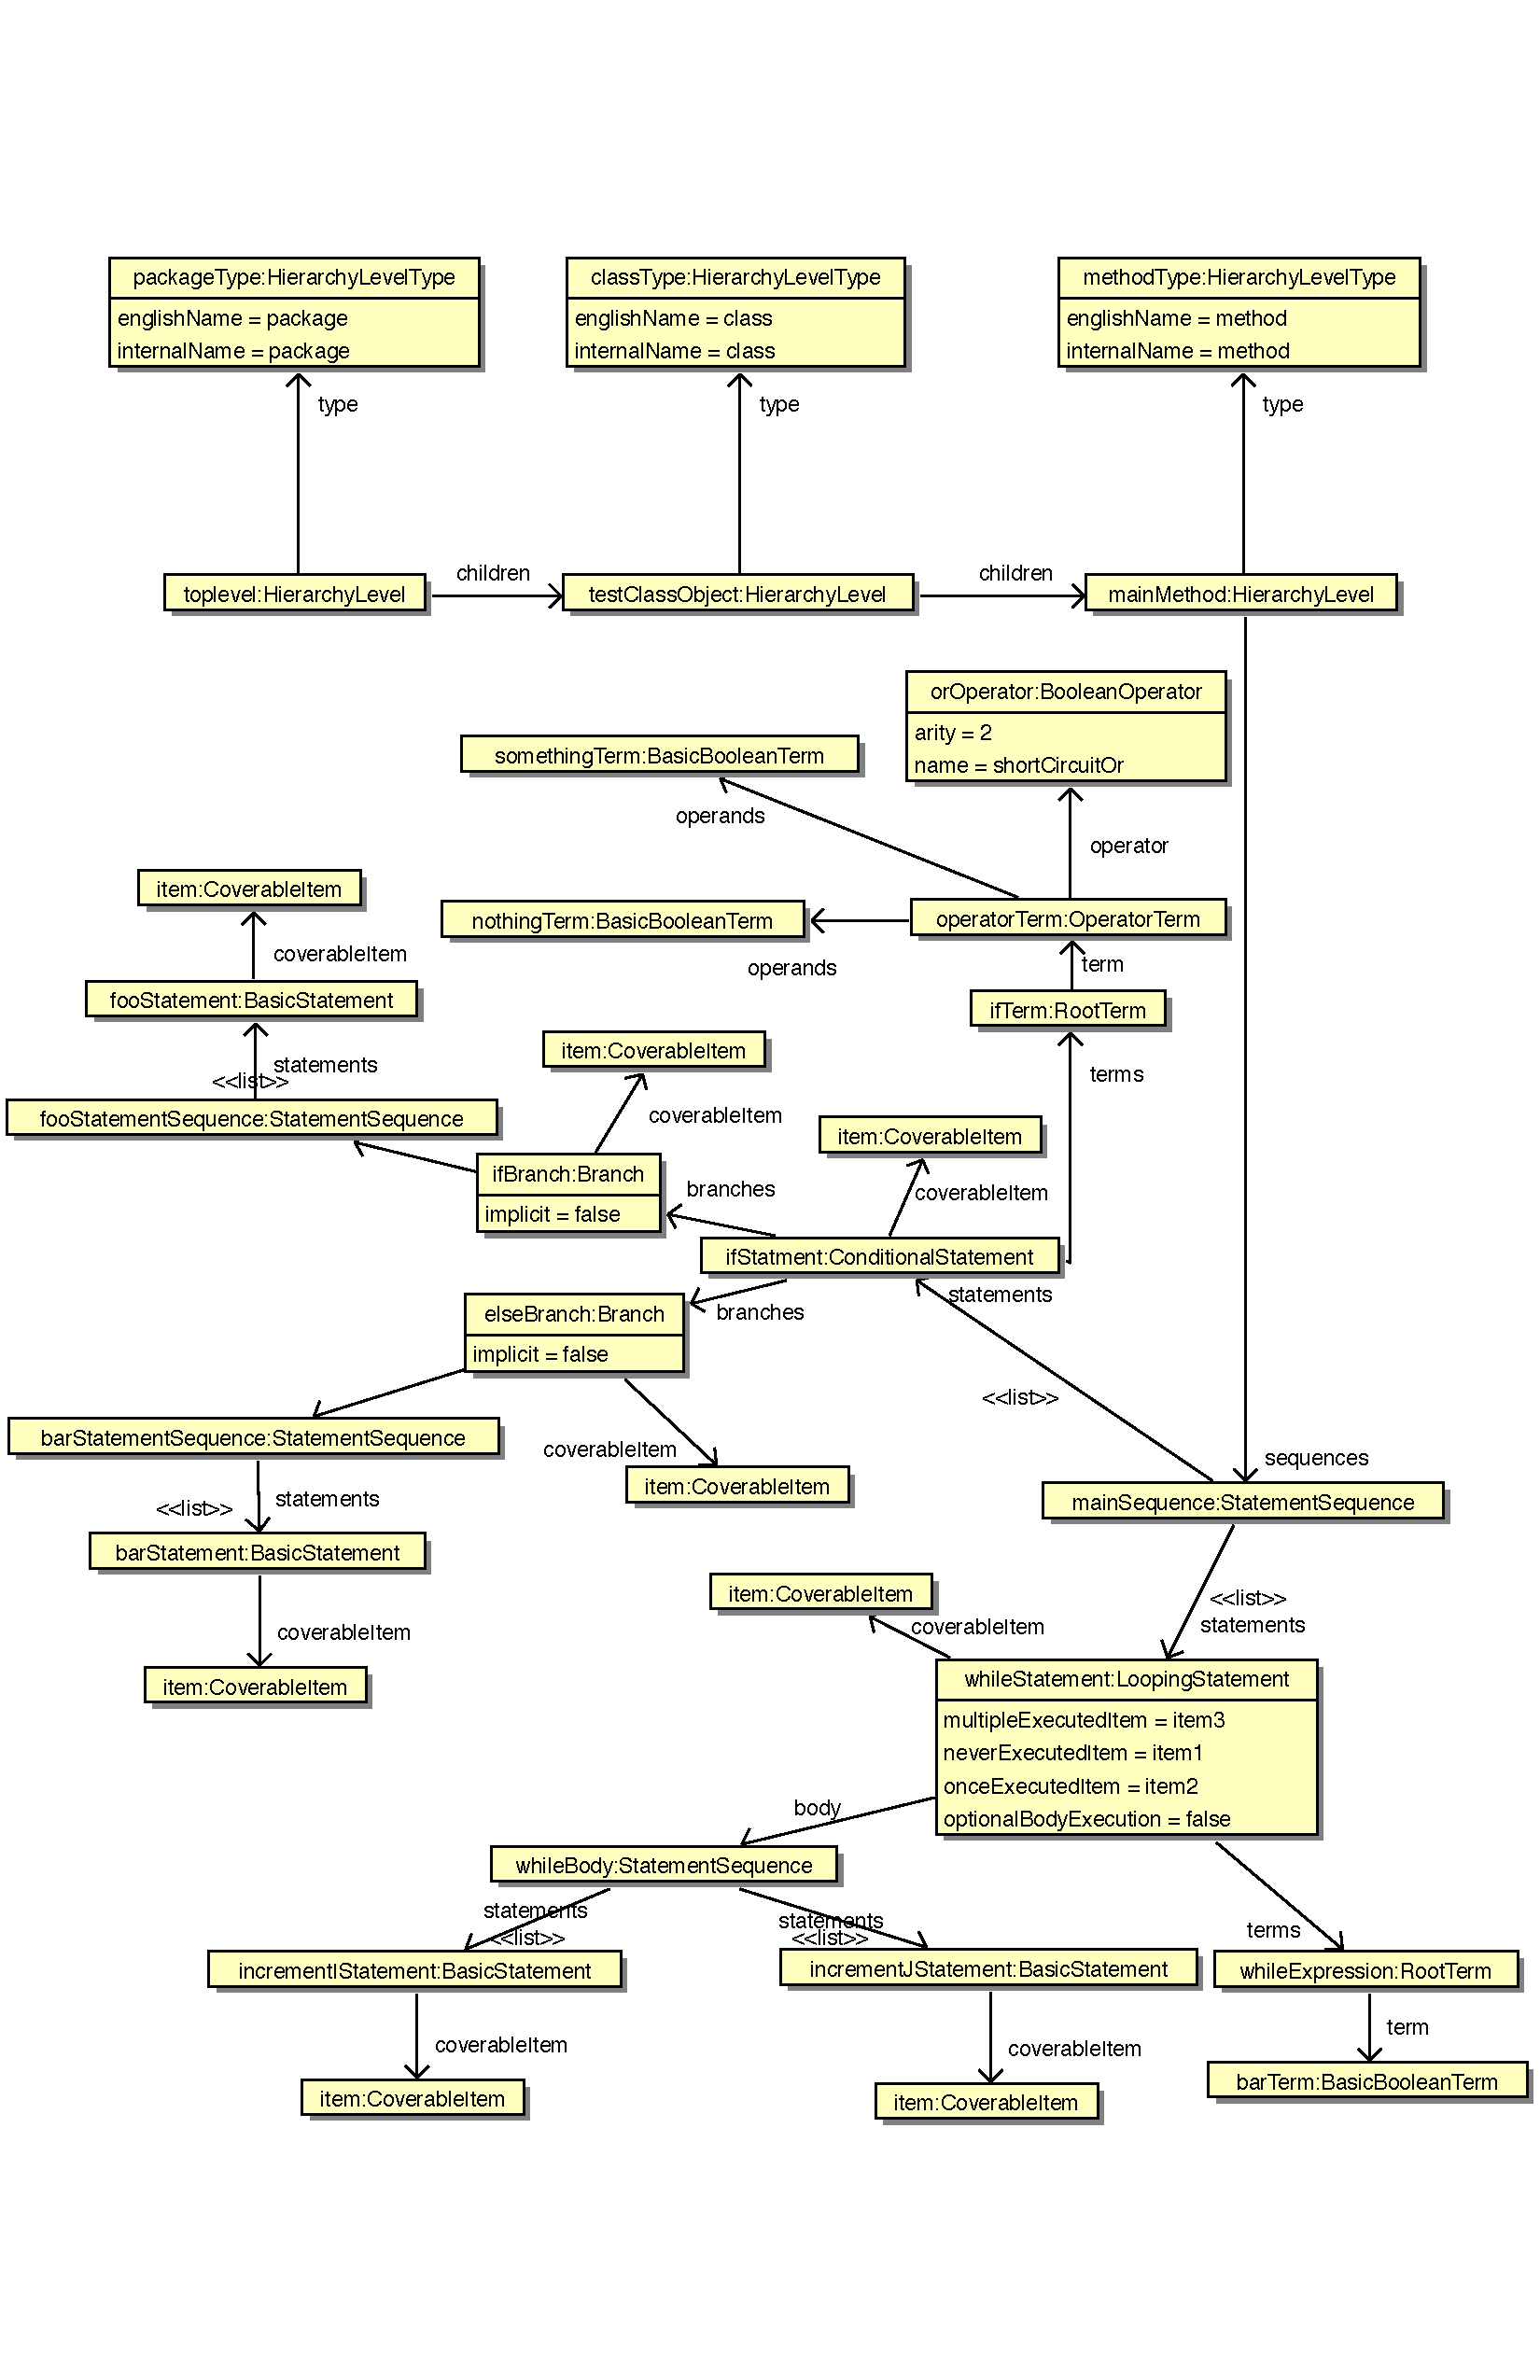
\includegraphics[width=\textwidth]{images/Model/example.pdf}
 \caption{Created object graph}
 \label{figure:Overview:ast_example}
\end{figure}

\clearpage
\subsection{Instrumentation}
\subsubsection{Overview}
This component includes all the packages and classes which deal with the instrumentation of source files. It includes all classes necessary to configure an instrumenter according to the users needs (e.g. select specific coverage criteria). All instrumenters are integrated using interfaces. A new instrumenter for a certain programming language must support these interfaces. The implementation will include instrumenters for Java 1.5 and COBOL-85.
The instrumentation component is modeled in greater detail in the detailed
design document.

\subsubsection{Instrumentation approach}
There are four coverage criteria: statement, branch, condition and loop coverage. The instrumentation for each criterion is independent. For that reason, the instrumentation approach is described separately using a pseudo programming language. All coverage data is captured using counters. These counters can be variables, fields or arrays. In the following examples, we use variables in the form \code{counter1} to represent the counters. All counters are stored persistently in the coverage log file, when a test case ends. The specification of the coverage log file can be found in appendix~\ref{Coverage log file specification} on page~\pageref{Coverage log file specification}.

\paragraph{Statement coverage}
In Java, the statement coverage has the semantic, that a statement is covered, if the programm flow \textbf{starts} to execute the statement. For this reason, a simple instrumentation before each statement is sufficient. The following example shows how statements are instrumented:
\newline\\
\begin{minipage}[t]{0.5\textwidth}
\begin{verbatim}

<statement1>


<statement2>


<statement3>
\end{verbatim}
\end{minipage}
\begin{minipage}[t]{0.5\textwidth}
\begin{verbatim}
counter1 := counter1 + 1
<statement1>

counter2 := counter2 + 1
<statement2>

counter3 := counter3 + 1
<statement3>
\end{verbatim}
\end{minipage}
\newline\\
In addition to the instrumentation of simple statements, looping and conditional statements are instrumented specially, see loop respectively branch coverage.

\paragraph{Branch coverage}
Branches are created by if, switch or similar statements. For each branch a counter is introduced. If a branch is omitted, like an else-branch, it is added with an appropriate counter. 
\newline\\
\begin{minipage}[t]{0.5\textwidth}
\begin{verbatim}
if <condition> then
  <statement sequence>
end if
\end{verbatim}
\end{minipage}
\begin{minipage}[t]{0.5\textwidth}
\begin{verbatim}
if <condition> then
  counter1 := counter1 + 1
  <statement sequence>
else
  counter2 := counter2 + 1
end if
\end{verbatim}
\end{minipage}
\newline\\\\
\begin{minipage}[t]{0.5\textwidth}
\begin{verbatim}
if <condition> then
  <statement sequence>
else
  <statement sequence>
end if
\end{verbatim}
\end{minipage}
\begin{minipage}[t]{0.5\textwidth}
\begin{verbatim}
if <condition> then
  counter3 := counter3 + 1
  <statement sequence>
else
  counter4 := counter4 + 1
  <statement sequence>
end if
\end{verbatim}
\end{minipage}
\newline\\\\
\begin{minipage}[t]{0.5\textwidth}
\begin{verbatim}
switch <variable>
  case <value> 
    <statement sequence>
  case <value> 
    <statement sequence>
end switch
\end{verbatim}
\end{minipage}
\begin{minipage}[t]{0.5\textwidth}
\begin{verbatim}
switch <variable>
  case <value> 
    counter5 := counter5 + 1
    <statement sequence>
  case <value> 
    counter6 := counter6 + 1
    <statement sequence>
  default
    counter7 := counter7 + 1
end switch
\end{verbatim}
\end{minipage}
\newline\\\\
\begin{minipage}[t]{0.5\textwidth}
\begin{verbatim}
switch <variable>
  case <value> 
    <statement sequence>
  case <value> 
    <statement sequence>
  default
    <statement sequence>
end switch
\end{verbatim}
\end{minipage}
\begin{minipage}[t]{0.5\textwidth}
\begin{verbatim}
switch <variable>
  case <value> 
    counter8 := counter8 + 1
    <statement sequence>
  case <value> 
    counter9 := counter9 + 1
    <statement sequence>
  default
    counter10 := counter10 + 1
    <statement sequence>
end switch
\end{verbatim}
\end{minipage}
\newline\\

\paragraph{Condition coverage}
The condition coverage instrumentation approach is highly dependent on the programming language. For example, short-circuit operators or side effects have to be considered. For programming languages without such characteristics the straight forward method which is shown here may be used.
\newline\\
\begin{minipage}[t]{0.5\textwidth}
\begin{verbatim}
if <conditionA> AND 
   <conditionB> then 
  <statement sequence>
end if
\end{verbatim}
\end{minipage}
\begin{minipage}[t]{0.5\textwidth}
\begin{verbatim}
if <conditionA> then
  if <conditionB> then
    counter11 := counter11 + 1
  else
    counter10 := counter10 + 1
  end if
else
  if <conditionB> then
    counter01 := counter01 + 1
  else
    counter00 := counter00 + 1
  end if
end if
if <conditionA> AND 
   <conditionB> then 
  <statement sequence>
end if
\end{verbatim}
\end{minipage}
\newline\\
For programming languages with side effects and short-circuit operators another approach is needed. See appendix~\ref{Formal Proof} on page~\pageref{Formal Proof} for details.
\newline\\

\paragraph{Loop coverage}
For each looping statement an auxiliary variable and three counter variables are introduced. The auxiliary variable is incremented for each run of the loop body. After the loop, the counter variable which corresponds to the value of the auxiliary variable is incremented.
\newline\\
\begin{minipage}[t]{0.5\textwidth}
\begin{verbatim}
while <condition> do
  <statement sequence>
end while
\end{verbatim}
\end{minipage}
\begin{minipage}[t]{0.5\textwidth}
\begin{verbatim}
auxiliary := 0
while <condition> do
  auxiliary := auxiliary + 1
  <statement sequence>
end while
switch auxiliary
  case 0 
    counter0 := counter0 + 1
  case 1 
    counter1 := counter1 + 1
  default
    counter2 := counter2 + 1
end switch
\end{verbatim}
\end{minipage}
\newline\\

\subsection{Metrics} \label{Components:Metrics}
This component contains the classes necessary to impose metrics on the data model. Furthermore all classes needed for the introduction of new metrics are provided as well. The implementation will include coverage metrics such as statement coverage, branch coverage, conditional coverage and loop coverage.

\subsection{Report}

\begin{figure}[hbtp]
 \centering
 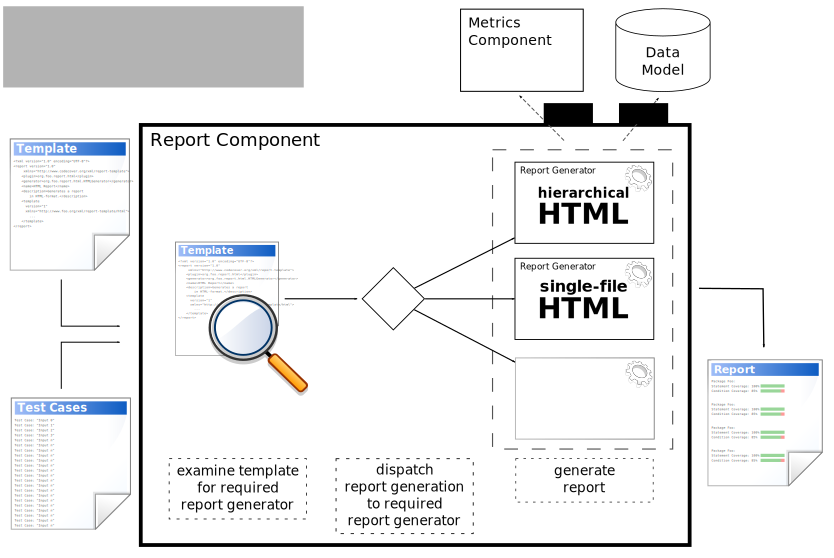
\includegraphics[width=\textwidth]{images/Report/report_process.pdf}
 \caption{Report generation}
 \label{figure:Components:Report:process}
\end{figure}

The report component consists of report generators whereas each of them is responsible for the creation of an output format, e.g. hierarchical HTML. A specific report is generated based on a template which specifies the report generator needed for report generation. The report component chooses the report generator which is able to process the template and dispatches report generation to the chosen report generator. That means for every report generator and thus for every output format exists a different template format.

An alternative to this design would have been to have only one specific template format for all types of output formats. But since output formats differ extensively in their structure and don't share many similarities the adjustements that could be set in templates would be very limited.

Another alternative would have been to generate an intermediate report which is transformed into the desired output format and document structure which are specified by templates. This templates, of course, would be specific to output format. The advantage of this alternative is that the generation of the raw data, which is saved in the intermediate report, is seperated from the generation of a specific output format. The problem is that the a powerful intermediate format has to be defined since the whole report component is based on it. And a mechanism would have to be implemented which transforms the intermediate report into the desired output format. But this is a difficult task which would consume too much time. An intermediate format which is already defined is DocBook. The DocBook report could be translated to the desired output format by using XSLT. But this means that templates would have to be defined in XSLT which is very complex and wouldn't comply with the requirement to allow easy adjustements to the design of reports.

Another alternative would have been to use an already existing report engine. But due to the lack of report engines which can produce hierarchically linked HTML reports (see~\ref{Components:Report:HTML}) this is not an option.

The report component needs the following input to generate a report:
\begin{itemize}
 \item the test cases which results are described by the report
 \item the template which specifies the design and output format of the report
 \item the structure of the code
 \item the coverage metrics for each code element (e.g. package, class)
 \item the original code
\end{itemize}

The \emph{test cases} are part of the data model and handed over to the report component when a report is requested.

The \emph{template} is a file in XML-format and is given to the report component when a report is requested. Templates are natural language specific. Although templates have a general structure (described in \ref{Components:Report:Template}), their detailed specification differs for each report generator.

The \emph{structure of the code} is needed to structure the report according to the code's structure. Thus the report component needs access to the data model which models the code's structure. 

To calculate the \emph{coverage metrics}, the metrics component is used. It receives test cases and a structural code element as input and then calculates the metrics by investigating the coverage log which is part of the data model.

The \emph{original code} is needed for code listings in reports.

\subsubsection{Programming language independency} \label{Components:Report:Independency:Programming}

Since the report component builds on the data model, which is language independent, the report component is language independent, too. The data model is hierarchically structured by \obj{HierarchicalLevel}s which build a tree. This tree structure can be used to map the code's structure on the structure of a report, that is the tree structure of the code builds the document structure of the report.

The data model identifies \emph{methods} for every programming language and SUT. The report component can use this information to place code listings with highlighting in the correct hierarchical level of the report's structure. Moreover this information can be used to decide which is the deepest level of the data model which will be mapped onto an own hierarchical level in the report. In case of the HTML report (see~\ref{Components:Report:HTML}) this means that it is possible to find out which structural code elements (namely methods) are described by code pages.

In Java the above mentioned \emph{methods}, of course, identify methods. In COBOL \emph{methods} identify sections.

\subsubsection{Natural language independency} \label{Components:Report:Independency:Natural}

Names of language specific types are saved for each structural code element. This makes it possible to output these language specific names (e.g., package, class, method in Java) to the report. The language specific names are saved in english. To generate a report in a different language, a template has to be created which translates the names. Thus templates are (natural) language specific.

\subsubsection{Template format} \label{Components:Report:Template}

The format of templates is XML and the general structure is as follows:
\begin{verbatim}
<?xml version="1.0" encoding="UTF-8"?>
<report version="1.0" xmlns="http://www.codecover.org/xml/report-template">
    <plugin>org.codecover.report.html</plugin>
    <generator>org.codecover.report.html.HTMLReportGenerator</generator>
    <name xml:lang="en">HTML Report (hierarchic)</name>
    <name xml:lang="de">HTML Report (hierarchisch)</name>
    <description xml:lang="en">
        Generates a hierarchical report in HTML-format.
    </description>
    <description xml:lang="de">
        Erstellt einen hierarchischen Report in HTML.
    </description>
    <template
      version="1"
      xmlns="http://www.codecover.org/xml/report-template/html-hierarchic">
    ...
    </template>
</report>
\end{verbatim}
All of the above defined elements and attributes are required in a template (none is optional). It is recommended but not required to use UTF-8 as the character encoding.

The element \code{plugin} defines the name of the plugin which contains an extension which is the report generator which can process the template. The extension is identified by the name contained in the element \code{generator}.
%\todo{Add reference to section about plugin management, if there will be one.}
% For details about the plugin management in \gbt see \ref{}.
In the above example the plugin which contains the report generator is named \code{org.codecover.report.html} and the report generator's name is \code{org.codecover.report.html.HierarchicalHTMLReportGenerator}.

The attribute \code{version} of the root element \code{report} sets the version of the template format. The template format which is specified in this document has the version 1.0. The version is compared to the internal version number of the report component. The major version number is incremented if a change in the component happens that requires restructuring the template format so that it is incompatible with the component before the change. If only minimal changes to the template format happen which don't affect the compatibility then the minor version number is incremented. This is the case if for example new elements are added to the template. An older version of the report component can't process these new elements but it still must be able to process the template and create a report. Changes to the structure inside the \code{template} element don't affect the version number because this structure is specific to the class which generates the report.

The namespace of the root element is defined in its attribute \code{xmlns} and must be \texttt{http://www.codecover.org/xml/report-template}.

The name of the template is set with the element \code{name} and a short description is set with the element \code{description}. The attribute \code{xml:lang} is used to indicate the language of the name and description. The values of the attribute are language identifiers as defined by RFC~4646\footnote{RFC 4646, Tags for the Identification of Languages: http://www.rfc-editor.org/rfc/rfc4646.txt}. The name and the description can be multiply defined with different language identifiers to supply the name and description in different languages. The Eclipse-Plugin can use this attribute to identify the name/description which language matches the one set in the GUI.

The attribute \code{version} of the element \code{template} sets the version of the template and is specific to the class which generates the report. It is recommended to use this version in the implementation of a report generating class to assure compatibility of the template and the class.

The content of the element \code{template} (indicated by \code{...} in the above example) is specific to the class which generates the report. Typically the element \code{template} contains a new level of subelements and these subelements contain CDATA-sections which contain the real templates with placeholders, see~\ref{Components:Report:HTML} for an example. The namespace of the element \code{template} is defined in its attribute \code{xmlns}. It must be unique and is recommended to be \texttt{http://www.codecover.org/xml/report-template/} plus a name of the output format of the template. For example the hierarchical HTML Report uses \texttt{html-hierarchic} as the name and the full namespace is \\
\texttt{http://www.codecover.org/xml/report-template/html-hierarchic}.

If the template is saved as a file in the filesystem the recommended filename is the name defined in element \code{name} whereas spaces are translated to underscores and potentially problematic characters like /, $\backslash$ and other non-basic latin letters should be avoided in the filename. The recommended file extension is \texttt{xml}. The filename for the hierarchical HTML Report is \texttt{HTML\_Report\_hierarchic.xml} for example.

\subsubsection{Extensibility}

The report component can be extended to support further output formats by implementing a new report generator and specifing a new template format.

Since the report component is independent from programming language, no costumization is needed to support new programming languages.

\subsubsection{Hierarchical HTML Report} \label{Components:Report:HTML}

% To be independent from programming languages, the data model internally identifies \emph{files} for every supported programming language. A file is an element in the code structure which directly contains codeThe first one is a \emph{container} for example a package in Java. A container can hold other containers or a \emph{code container}. A code container (e.g., a file in COBOL or a file or a class in Java) directly contains code (containers do not contain code directly). The data model is hierarchically organized that is the top most code containers in the hierarchy can be identified. These top most code containers (e.g., files in Java) can be used to build the code pages in a hierarchical HTML report for example.

\paragraph{Structure}

The hierarchical HTML Report consists of three types of pages which are described in the specification. This document only describes how the hierarchical HTML report generator maps the structure of the data model onto the structure of the report.

Every report has exactly one title page. It lists the topmost elements of the hierarchical code structure. Every listed element is linked to its corresponding detail page. A detail page is either a selection page or a code page.

All elements above the level of methods (see~\ref{Components:Report:Independency:Programming}) are described in selection pages. Selection pages describe their corresponding element and contain a list of the direct children of the corresponding element. Every listed element is linked to its corresponding detail page. Methods are described in code pages which are the deepest hierarchical level of the hierarchical HTML report.

In Java the only structural types above the level of methods are packages and classes which are described in selection pages.

\begin{figure}[hbtp]
 \centering
 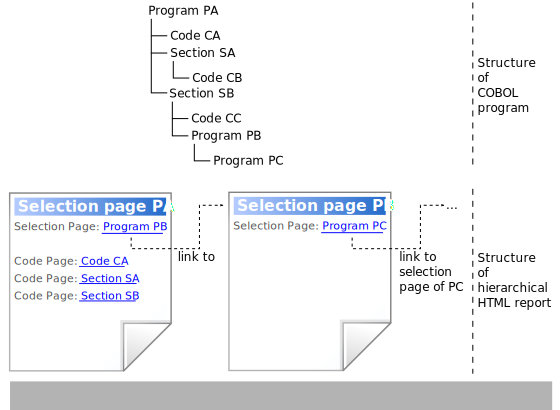
\includegraphics[width=0.85\textwidth]{images/Report/hierarchical_html_cobol.pdf}
 \caption{Structure of hierarchical HTML report of COBOL programs}
 \label{figure:Components:Report:COBOL}
\end{figure}

In COBOL methods, which are described by code pages, are sections. COBOL-programs, which can be nested to arbitrary depth, are described by selection pages. If a program contains code without an enclosing section, it is described in an extra code page which is put on the same level (in the report) as the code pages of the sections of the program.

To avoid redundancy of code listings, the code of sub-programs is omitted in code pages. For example in the report of figure \ref{figure:Components:Report:COBOL} the code page of section SB wouldn't neither contain the code of program PB nor PC. The selection page for program PC and the code pages of code CA, section SA and SB are omitted in figure \ref{figure:Components:Report:COBOL} but they would exist in the real report of course.


\paragraph{Generation} \label{Components:Report:HTML_hierarchic:Generation}

Generating a report is basically done by traversing the tree structure of the data model and generating the corresponding selection or code page for each element of the tree. Every page contains metrics about its corresponding element. To calculate these metrics, the hierarchical HTML report generator uses the metrics component (see~\ref{Components:Metrics}).

Apache Velocity\footnote{Apache Velocity: http://velocity.apache.org/} is used as the template engine. This works as follows:
\begin{enumerate}
\item An instance of the Apache Velocity template engine is created.
\item A so-called Context is filled with the data that will be inserted into the template HTML code for the title page. The inserted data is for example the achieved statement coverage for the whole SUT or the names of the top-level packages (if it's a report about a Java SUT). To fill the Context, the actual value and a key to this value are saved. The key of the value is the name of the placeholder in the template HTML code.
\item The template HTML code is \emph{merged} with the Context, that is the placeholders are replaced with the real data.
\item Now a Context is created for each selection page. In case of Java it is a Context for each package and class. In case of COBOL it is a context for each program.
\item The Contexts are merged with the template HTML code for selection pages. This creates the selection pages of the report.
\item Now a Context is created for each code page, that is for each method (see~\ref{Components:Report:Independency:Programming}).
\item The Contexts are merged with the template HTML code for code pages. This creates the code pages of the report.
\end{enumerate}

\paragraph{Template format}

The template format is extended as follows:
\begin{verbatim}
<?xml version="1.0" encoding="UTF-8"?>
<report version="1.0" xmlns="http://www.codecover.org/xml/report-template">
    <plugin>org.codecover.report.html</plugin>
    <generator>org.codecover.report.html.HierarchicalHTMLReportGenerator</generator>
    <name xml:lang="en">HTML Report (hierarchic)</name>
    <name xml:lang="de">HTML Report (hierarchisch)</name>
    <description xml:lang="en">
        Generates a hierarchical report in HTML-format.
    </description>
    <description xml:lang="de">
        Erstellt einen hierarchischen Report in HTML.
    </description>
    <template
      version="1"
      xmlns="http://www.codecover.org/xml/report-template/html-hierarchic">
        <language>de</language>
        <title-page><![CDATA[
            ...
        ]]></title-page>
        <selection-page><![CDATA[
            ...
        ]]></selection-page>
        <code-page><![CDATA[
            ...
        ]]></code-page>
        <text-file filename="style.css" content-type="text/css"><![CDATA[
            ...
        ]]></text-file>
        <resource filename="logo.png">...</resource>
    </template>
</report>
\end{verbatim}
The filename of the template is \texttt{HTML\_Report\_hierarchic.xml}.

The version number defined in the attribute \code{version} of element \code{template} must be incremented if any changes to the HTML report generation happen that affect the structure or semantics of placeholders inside the element \code{template}.

The element \code{language} identifies the language of the generated report and is a two-letter code according to ISO~639-1.

There are three new elements which contain the template HTML code for title (\code{title-page}), selection (\code{selection-page}) and code pages (\code{code-page}). The HTML code of the template contains placeholders for the data which will be inserted in the template by Apache Velocity.

The two elements \code{text-file} and \code{resource} are used to provide additional text files and binary resources. The \code{text-file}-element contains the text (e.g., a CSS stylesheet) which is to be written into a text file with the content type specified in the attribute \code{content-type}. The \code{resource}-element contains the content of a binary file encoded in Base64\footnote{Base64 is specified in RFC~4648: ftp://ftp.rfc-editor.org/in-notes/rfc4648.txt}. Both elements have the attribute \code{filename} which denotes the path to the file relative to the output directory of the report.
% I know that CSS already contains the word "stylesheet". But I think "CSS stylesheet" is more prevalent than "Cascading Stylesheet" (most people probably heard of CSS rather than Cascading stylesheets). [Robert]

\subsubsection{Single-file HTML Report} \label{Components:Report:HTML_singlefile}

\paragraph{Structure}

This type of report consists of only one HTML page. It is divided into an overview section and a code section. The overview section lists the units (e.g. classes, methods) of the SUT and their corresponding metrics. Moreover it contains some statistics on the structure of the SUT (e.g., the number of classes) and information about the test cases the report is about.  The code listings of all source files are contained in the code section. 

\paragraph{Generation}

To generate the single-file HTML report nearly the same procedure as described in \ref{Components:Report:HTML_hierarchic:Generation} is used. The only difference is that only one Context is created which contains the data to be inserted into the template of the file.

\paragraph{Template format}

The template format is extended as follows:
\begin{verbatim}
<?xml version="1.0" encoding="UTF-8"?>
<report version="1.0" xmlns="http://www.codecover.org/xml/report-template">
    <plugin>org.codecover.report.html</plugin>
    <generator>org.codecover.report.html.SingleFileHTMLReportGenerator</generator>
    <name xml:lang="en">HTML Report (single-file)</name>
    <name xml:lang="de">HTML Report (eine Datei)</name>
    <description xml:lang="en">
        Generates a single-file report in HTML-format.
    </description>
    <description xml:lang="de">
        Erstellt einen Report in einer einzigen HTML-Datei.
    </description>
    <template
      version="1"
      xmlns="http://www.codecover.org/xml/report-template/html-single-file">
        <language>de</language>
        <html-page><![CDATA[
            ...
        ]]></html-page>
    </template>
</report>
\end{verbatim}
The filename of the template is \texttt{HTML\_Report\_SingleFile.xml}.

The version number defined in the attribute \code{version} of element \code{template} must be incremented if any changes to the report generation happen that affect the structure or semantics of placeholders inside the element \code{template}.

The element \code{language} identifies the language of the generated report and is a two-letter code according to ISO~639-1.

The template HTML code is defined with the element \code{html-page}.

\subsection{Batch}

This component encompasses all the packages and classes necessary for the command line interface.

\subsection{Eclipse}

\def\extpoint#1{
\code{\texorpdfstring{\url{org.eclipse.#1}}{org.eclipse.#1}}
}

This component contains all the packages and classes which are related to the Eclipse plugin part of \gbt.

%The Eclipse plugin component mainly provides a GUI. See the detailed design document for a list of Eclipse related packages and Eclipse Extension Points which will be used.

\subsubsection{Data management}

The classes and interfaces mentioned in this section are contained in the package \pkg{org.codecover.eclipse.tscmanager} except for the class \cls{TestSessionContainer} which is contained in the package \pkg{org.codecover.model}.

\paragraph{Terminology}

The Eclipse plugin of \gbt can handle multiple test session containers. Each test session container is associated with a specific project in Eclipse. Eclipse projects are stored in the \emph{workspace} of Eclipse. The files of the test session containers are stored in the \emph{\gbt-folder} of the associated project. The \emph{\gbt-folder} is a folder on the root level of each Eclipse project which contains test session containers. Thus the user just has to copy the folder of an Eclipse project to get a full backup of the project including his coverage measurements.

A Test session container which is associated with a currently \emph{open} project is called a \emph{known test session container}. The reason for this term is that files and folders which reside in closed projects aren't accessible and thus can't be "known" by the plugin.

The \emph{active test session container} is the known test session container which contains the \emph{active test cases} which are currently visualized in the plugin's views, e.g. the Coverage view and the Test Sessions view. The \emph{active test cases} can be selected in the Test Sessions view, see the specification document for details.

A \emph{test element} is either a test session or a test case.

\paragraph{TSContainerManager}

The central component which handles the data management in the Eclipse plugin is the \cls{TSContainerManager} which provides the following functions:
\begin{itemize}
\item Providing methods to select the active test session container and the active test cases
\item Providing access to the currently active test session container (to add/delete/modify test elements)
\item Providing the currently active test cases
\item Providing a list of the currently known test session containers
\item Providing methods to add and delete test session containers
\item Notification of listeners (e.g., the views of the plugin) about changes
\item Saving and loading the test session containers
\item Saving and loading which test cases are active
\end{itemize}

\subparagraph{Storing the test session containers}

The implemented concept of handling multiple test session containers with the Eclipse plugin is simple. As mentioned before each test session container is associated with a project and stored in the \gbt-folder of this project. This means adding a test session container to a project is as simple as copying the file to the \gbt-folder of the project.

On startup of the plugin the \cls{TSContainerManager} scans all \gbt-folders of all open projects and loads all files of the \gbt-folders once to determine which test session containers they contain. Since holding all test session containers in memory would consume to much memory, only a representation of each found test session container is stored in the \cls{TSContainerManager}. This representation is an object of class \cls{TSContainerInfo} and stores the following information about the represented test session container:
\begin{itemize}
\item the path to the file of the test session container
\item the associated project
\item the creation date of the test session container
\item the names of the active test cases of the test session container
\end{itemize}
The path is used as a unique ID for each test session container and makes it possible to distinguish known test session containers from each other.

The managed list of known test session containers can of course change during the execution of the plugin if:
\begin{itemize}
\item the user opens a project: the newly accessible test session containers are added to the list
\item the user closes a project: the test session containers contained in (associated with) the project are removed from the list
\item the user creates a test session container by running a coverage measurement: the test session container is added to the list
\item the user imports a test session container into a project: the test session container is added to the list
\item the user deletes a test session container: the test session container is removed from the list
\end{itemize}
The first two cases are detected by listening to changes in the workspace of Eclipse, which is done by \cls{WorkspaceListener}, and then taking the appropriate action (adding/removing). The other three cases are detected by the \cls{TSContainerManager} itself because adding and deletion of test session containers are handled by the \cls{TSContainerManager}.

\subparagraph{Active test session container}

As mentioned before it would be too resource-consuming to hold all known test session containers in memory, which is the reason why only the active test session container is actually represented by an object of class \cls{TestSessionContainer} and can be modified. To avoid inconsistencies the \cls{TSContainerManager} provides this \obj{TestSessionContainer} as a compound together with the respective \obj{TSContainerInfo}-representation and the active test cases in the form of an object of class \cls{ActiveTSContainerInfo}.

Activating an other test session container is done by passing the \cls{TSContainerManager} the \cls{TSContainerInfo}-representation of the test session container to activate. The \cls{TSContainerManager} then loads the test session container from its file into memory.

% Modification of the active test session container includes adding/deleting test elements and changing the name and comment of test elements.
Since Eclipse is a multi-threaded application, the plugin has to take care of concurrent modifications. To apply changes to the active test session container one has to provide an \cls{ActiveTSContainerRunnable} which is then passed to the \cls{TSContainerManager} and synchronized with other modifications to the active test session container.

\subparagraph{Active test cases} \label{Overview:Eclipse:Data_management:Active_test_cases}

The active test cases can be selected by a component of the plugin by passing a set of test cases to the \cls{TSContainerManager}. In the perspective of the \cls{TSContainerManager} the active test cases are just a set of test cases of the currently active test session container, which are provided to the components of the plugin which visualize them.

To be able to "remember" the active test cases of a test session container after an other test session container was activated, the names of the active test cases are stored in the \cls{TSContainerInfo}-representations of the known test session containers as objects of class \cls{TestCaseInfo}. When a test session container is activated the set of active test cases can be restored by reading the stored names (the \obj{TestCaseInfo} objects) from the \cls{TSContainerInfo}-representation. This information is also stored on disk by \cls{ActiveTestCasesStorage} and \cls{ActiveTestCasesSaveParticipant} to be able to "remember" the active test cases after a restart of the plugin. 

\subparagraph{Listeners}

There are two ways to access the information managed by the \cls{TSContainerManager}. One way is to actively get the information by calling the methods of \cls{TSContainerManager}. The passive approach is to register a component as a listener, which is then notified of changes in the \cls{TSContainerManager}. Listeners, which must implement the interface \itf{TSContainerManagerListener}, are informed about changes of:
\begin{itemize}
\item the selection of the active test session container
\item the active test session container itself (e.g., deletion of a test case)
\item the selection of active test cases (of the active test session container)
\item the list of known test session containers (i.e., a test session container was added / removed)
\end{itemize}
The listeners are handled by the \cls{TSContainerManagerListenerHandler}.

\subparagraph{Saving and loading}

The easiest way of implementing the saving of test session containers, that is the process of writing them to disk, would have been to perform a save instantly after a change had been performed. Since saving is a resource-consuming operation, this approach isn't feasible. To achieve the goal of minimizing save operations, saving is only performed when an other test session container is activated or the associated project is closed. Since only the active test session container is kept in memory, the save operation can't be deferred any further (else the changes would be lost).

The actual operation of reading and writing the files of the test session containers is already implemented by the class \cls{TestSessionContainer} and called by the class \cls{TSContainerStorage} which handles loading and saving of test session containers.

For saving test session containers when a project is closed, a special treatment has to be undertaken because during the close-event (propagated by Eclipse) the workspace is locked for changes and thus saving, which implicates a modification of the workspace, can't be performed. Therefore the save operation is queued in the \cls{TSContainerSaveQueue} until Eclipse requests the plugin to perform saving. This request can be detected by implementing a \pkg{org.eclipse.core.resources.}\imp{ISaveParticipant} which is then registered to receive save requests from Eclipse. \cls{TSContainerManagerSaveParticipantHandler} is the class which receives the requests and distributes them to all registered \imp{SaveParticipants}. The two save participants are the \cls{TSContainerSaveParticipant} and the \linebreak\cls{ActiveTestCasesSaveParticipant}. The former saves the active test session container if it changed since it was last saved and furthermore performes the save operations queued in the \cls{TSContainerSaveQueue}. The latter saves which test cases are active (see~\ref{Overview:Eclipse:Data_management:Active_test_cases}) and which test session container is active.

\subsubsection{Build and Run}

This section covers the parts of the Eclipse plugin which are relevant for
the build of the instrumented SUT, its execution and necessary post-processing.

\paragraph{Building the instrumented SUT}
\gbt doesn't do incremental instrumentation yet, so whenever a
build is triggered by Eclipse a full build needs to be done.
The build process of an instrumented SUT basically works like this:
\gbt participates in the build of the uninstrumented SUT
with the help of \cls{CodeCoverCompilationParticipant}, which
allows \gbt to perform additional actions before the actual build
This includes searching for a test session container which 
matches the current code base, or creating a new one if necessary.
As a second step the instrumentation of the sources is also performed there. The
instrumented sources are placed in a project dependent location in the
metadata section of the workspace. Last step is the compilation of the
instrumented sources by invoking the Eclipse java compiler
with the compiler settings of the project.

\paragraph{Running the instrumented SUT}
The compiled instrumented SUT has been placed in a project dependent
location in the workspace metadata section by the
\cls{CodeCoverCompilationParticipant}. In order to execute the
instrumented object code, a redirection from the uninstrumented object
to the instrumented object code needs to be performed.
This is done with help of the
\cls{CodeCoverClasspathProvider} which adds another classpath entry to
the top of the list of classpath entries which points to the directory
where the instrumented object code is stored. Since the java runtime
searches for classes in the order of the classpath entries, the
instrumented classes will be found first, leading to the execution of
the instrumented SUT. A \cls{ClasspathProvider} is bound to a specific
launch configuration. By using the \cls{CodeCoverTab}, which is
added to the list of tabs which are shown for a launch configuration,
the user is able to set and unset the \cls{CodeCoverClasspathProvider}
for the opened launch configuration and thereby be able to quickly
switch between runs of the instrumented and uninstrumented SUT.

\paragraph{Post-execution actions}
After the termination of a SUT certain actions need to be performed.
One important action is the import of the coverage log which
resulted from the execution of the SUT. In order to track the
execution of a SUT a \cls{CodeCoverDebugListener} is registered with
Eclipse. On SUT termination \cls{CodeCoverDebugListener}
receives a respective event. This event triggers functionality
which searches for a test session container to whom the coverage log
belongs to. In case the search is successful, the coverage log is
imported into the test session container and the views are updated
to show the new data.

\subsubsection{Annotation}

The classes and interfaces described in this section are contained in the
package \pkg{org.codecover.eclipse.annotation}. Other classes are mentioned
with their qualified names where they could be confused easily.

This package adds coverage highlighting of the active test cases to the default
java editor of eclipse. This is done by attaching an implementation of
\imp{org.eclipse.jface.text.source.IAnnotationModel} to every java editor as it is opened. The model then
queries the \pkg{org.codecover.report} to find out what information to annotate
where. It adds an \cls{org.eclipse.jface.text.source.Annotation} to the editor
for each consecutive region of text to be highlighted in a certain way. The
layout of these annotations is defined via
\extpoint{ui.editors.markerAnnotationSpecification}.

\paragraph{Attaching the model}
The \cls{org.codecover.eclipse.CodeCoverPlugin} makes sure that an instance of
\linebreak \cls{EditorTracker} exists while the plugin is running. \cls{EditorTracker}
registers listeners with Eclipse to get informed whenever a
\imp{org.eclipse.ui.IWorkbenchPart} is created. For every
\imp{org.eclipse.ui.texteditor.ITextEditor} that is opened it calls
\code{CoverageAnnotationModel.attach(...)}, which adds a new instance of
\linebreak\cls{CoverageAnnotationModel} to the editors
\imp{org.eclipse.jface.text.source.}\linebreak\imp{IAnnotationModelExtension}. From then on
all annotations provided by this model will be displayed among the usual
annotations that editor displays.

\paragraph{The annotation model}
\cls{CoverageAnnotationModel} implements an annotation model to serve \linebreak\cls{EclPositionedAnnotation}s
to the editor. They are subclassed as required to show every kind of highlighting including hotpath.
The model is also responsilbe for deciding when and what to annotate.

\cls{CoverageAnnotationModel} listens for changes in the document and in the data model of
\gbt. On every change it uses \cls{org.codecover.eclipse.utils.}
\linebreak\cls{EclipseMastLinkage} to find the corresponding \cls{SourceFile} to the
\cls{ICompilationUnit} % unqualified elcipse class
displayed in the editor. If it finds a SourceFile and it's content is equal to the editor's content the file is annotated.

The \mtd{CoverageAnnotationModel.createAnnotations()} is responsible for querying the model what
to annotate and creating all \cls{EclPositionedAnnotation}s the user sees. To measure the coverage
of source files it queries \cls{org.codecover.highlighting.}\linebreak
\cls{CodeHighlighting}. Currently it just
converts the results of \mtd{annotateCoverage(...)}
and \mtd{generateLineAnnotationsByFile()}
into \cls{EclPositionedAnnotation}s.

\pagebreak
\emph{Don't confuse} the annotations subclassing \cls{org.eclipse.jface.text.source.}
\linebreak\cls{Annotation}
with those in \pkg{org.codecover.report.highlighting.annotation}.  The \emph{former}, prefixed
with Ecl, are those you see in your Eclipse editor. The \emph{latter} make up the source file oriented
view of what characters were covered how, using a specific set of metrics and test cases.

\paragraph{Layout of annotations}
In Eclipse every \cls{org.eclipse.jface.text.source.Annotation} has a type string that is defined
in \code{plugin.xml}. This type decides which layout is used to display the annotation in the editor.

There are two kinds of annotations displayed in Eclipse. The first is \cls{EclCoverageAnnotation}
which is used to show the user which elements are covered. The type of these annotations has the
form \code{org.codecover.eclipse.annotation.*Coverage*Annotation}. At the first \code{*} the level
of coverage is inserted (one of \code{full}, \code{partial} and \code{no}). At the second \code{*}
the kind of coverage metric is inserted (one of \code{Other} -- for user defined metrics -- and
\code{Branch}, \code{Conditional}, \code{Loop} and \code{Statement} -- for the bundled metrics).
All of these annotations have their default color layout defined in \code{plugin.xml} and are
defined to be configurable individually in the Eclipse preferences dialog.

The second kind of annotation is \cls{hotpath.EclLineExecutionAnnotation} which is used to 
show the hot path icons in the editor. It's type is
\code{org.codecover.eclipse.annotation.}\linebreak\code{lineExecutionAnnotation}. The class
\cls{LineExecutionImageProvider} generates the icons the user sees based on
the attributes of \cls{hotpath.EclLineExecutionAnnotation}. The mapping
between annotation and color is implemented in
\mtd{generateIcon}\linebreak\mtd{(EclLineExecutionAnnotation)}.

\clearpage
\subsection{Package overview}

\begin{figure}[hbtp]
 \centering
 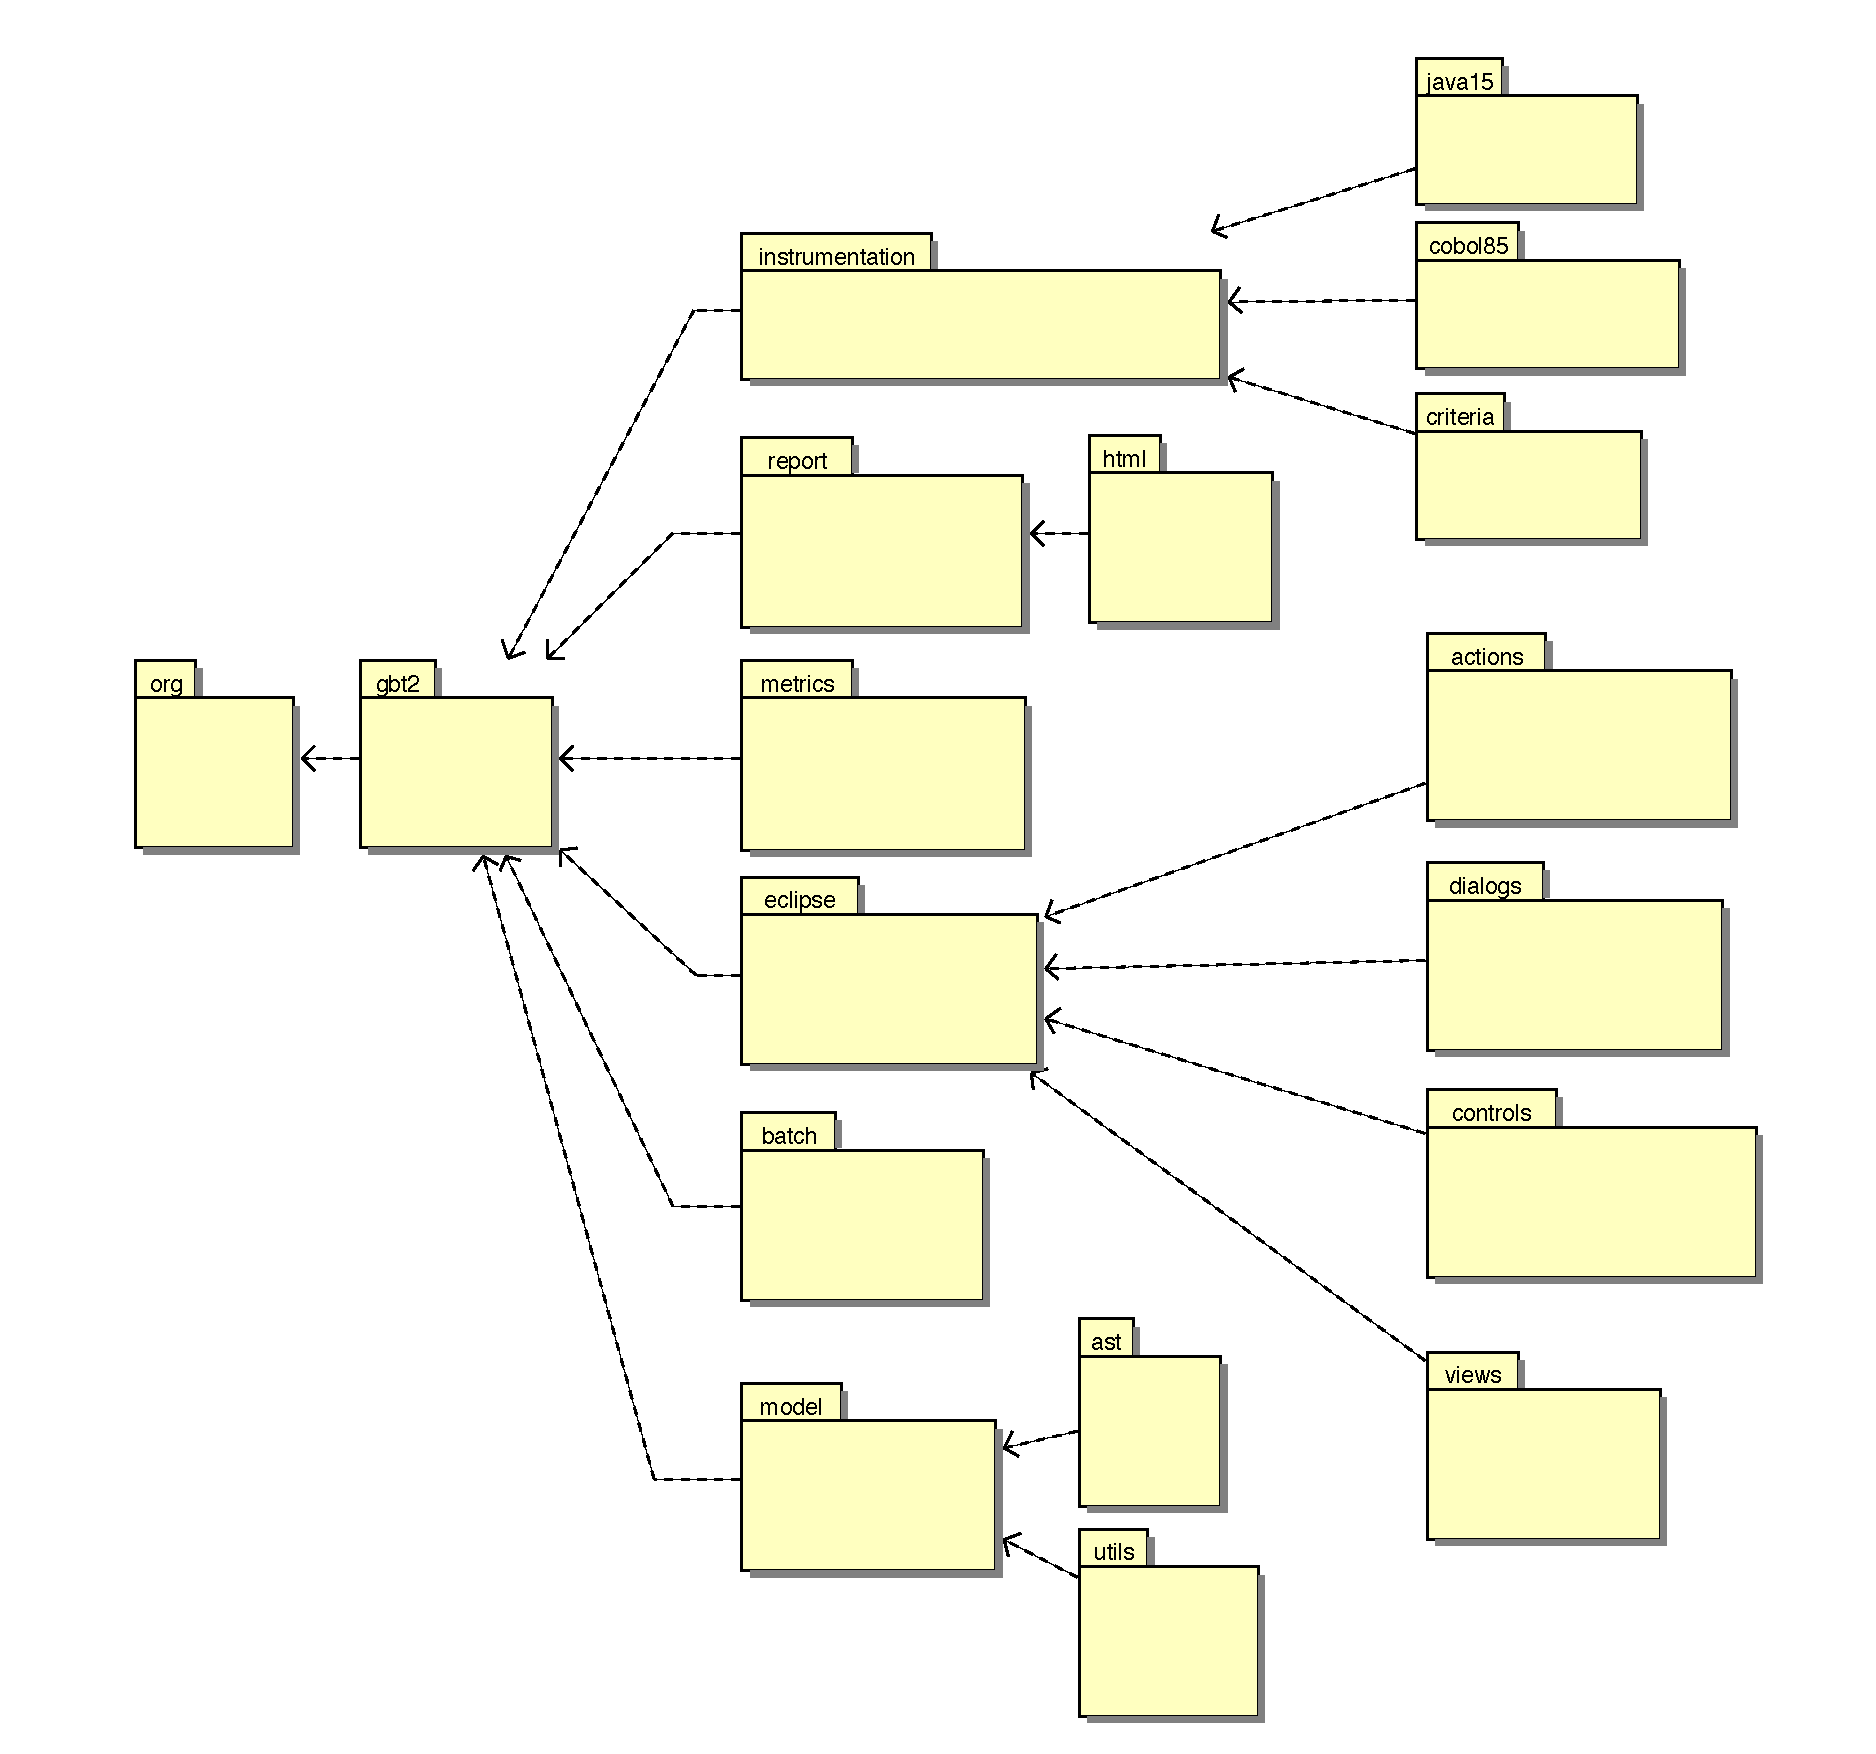
\includegraphics[width=\textwidth]{images/Overview/package_overview.pdf}
 \caption{Package overview}
 \label{figure:Overview:package_overview}
\end{figure}

This section provides an overview of the deployment plan of the software. The domain used for the development of the software is used as the common root for the packages, meaning all packages are in the \pkg{\rootpkg} namespace.  As seen in figure~\ref{figure:Overview:package_overview} the components from section~\ref{Component_Overview} are represented as the six main packages. They are further refined through packages of their own, e.g. the packages for the java instrumentation (\pkg{java15}) and the COBOL instrumentation (\pkg{cobol85}).
